
\begin{tikzpicture}[remember picture,overlay,inner sep=0pt,outer sep=0pt]
	\node at (current page.center) {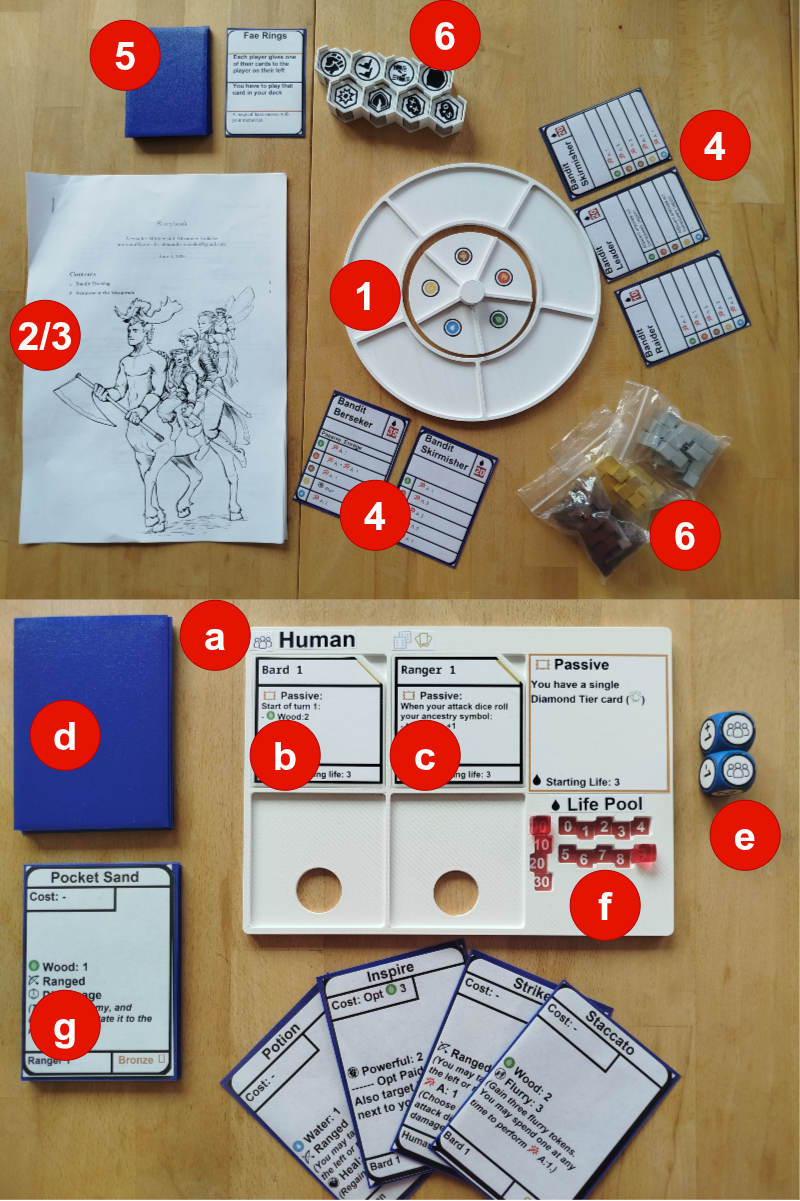
\includegraphics[width=0.9\paperwidth]{../ExplanationPics/Setup_Board.drawio.png}};
\end{tikzpicture}

\newpage

\section{Setup}
\subsection{Common setup}

\begin{minipage}[t][4cm][t]{1\textwidth}
\vspace{0.3cm}
To create the shared space in the middle, set up the following items:
\begin{enumerate}
	\item \textbf{Wheel} - Put the Wheel of Elements in the middle.
	\item \textbf{Storybook} - Select a new story from the storybook (we recommend story no.1 "Bandit Tracking" if it is everyone's first time playing).
	\item \textbf{Story} - Read out the first passage of the story.
	\item \textbf{Encounter} - Set up the enemies corresponding to the first encounter.
	\item \textbf{Event Deck} - Place the event deck to the side, may optionally be used in encounters 2\&3.
	\item \textbf{Markers} - Place the tracking cubes and markers on the side.
\end{enumerate}

\end{minipage}	



\subsection{Player setup}

\begin{minipage}[t][6cm][t]{1\textwidth}
	To construct their first action and modifier deck, each \textbf{player} follows these steps:
	\begin{enumerate}[a)]	
		\item \textbf{Ancestry} - Pick an ancestry and take it's tableau.
		\item \textbf{Class 1} - Pick your first rank 1 class and place its tile into the tableau.
		\item \textbf{Class 2} - Pick a second (different) rank 1 class and place its tile into the tableau.
		\item \textbf{Action Deck} - Shuffle all action cards from your ancestry and two classes together. This forms your action deck.
		\item \textbf{Attack Dice} - Take the blue and red attack dice from your ancestry, as indicated by the tableau.
		\item \textbf{Starting Life} - Calculate your starting life by adding all values from your ancestry tableau and the two classes. Place a life marker on the corresponding position.
		\item \textbf{Action Discard Pile} - Designate a space to place cards after you play them.
	\end{enumerate}
\end{minipage}	

\begin{tcolorbox}[colframe=blue, colback=white]
	Reminder -	There is no need (yet) to get hung up on your class choices, just pick something funny.
\end{tcolorbox}
%\fbox{\parbox[4cm]{\textwidth}{Picture:  Silverkin, sorting stacks of archaic thick playing cards}}


%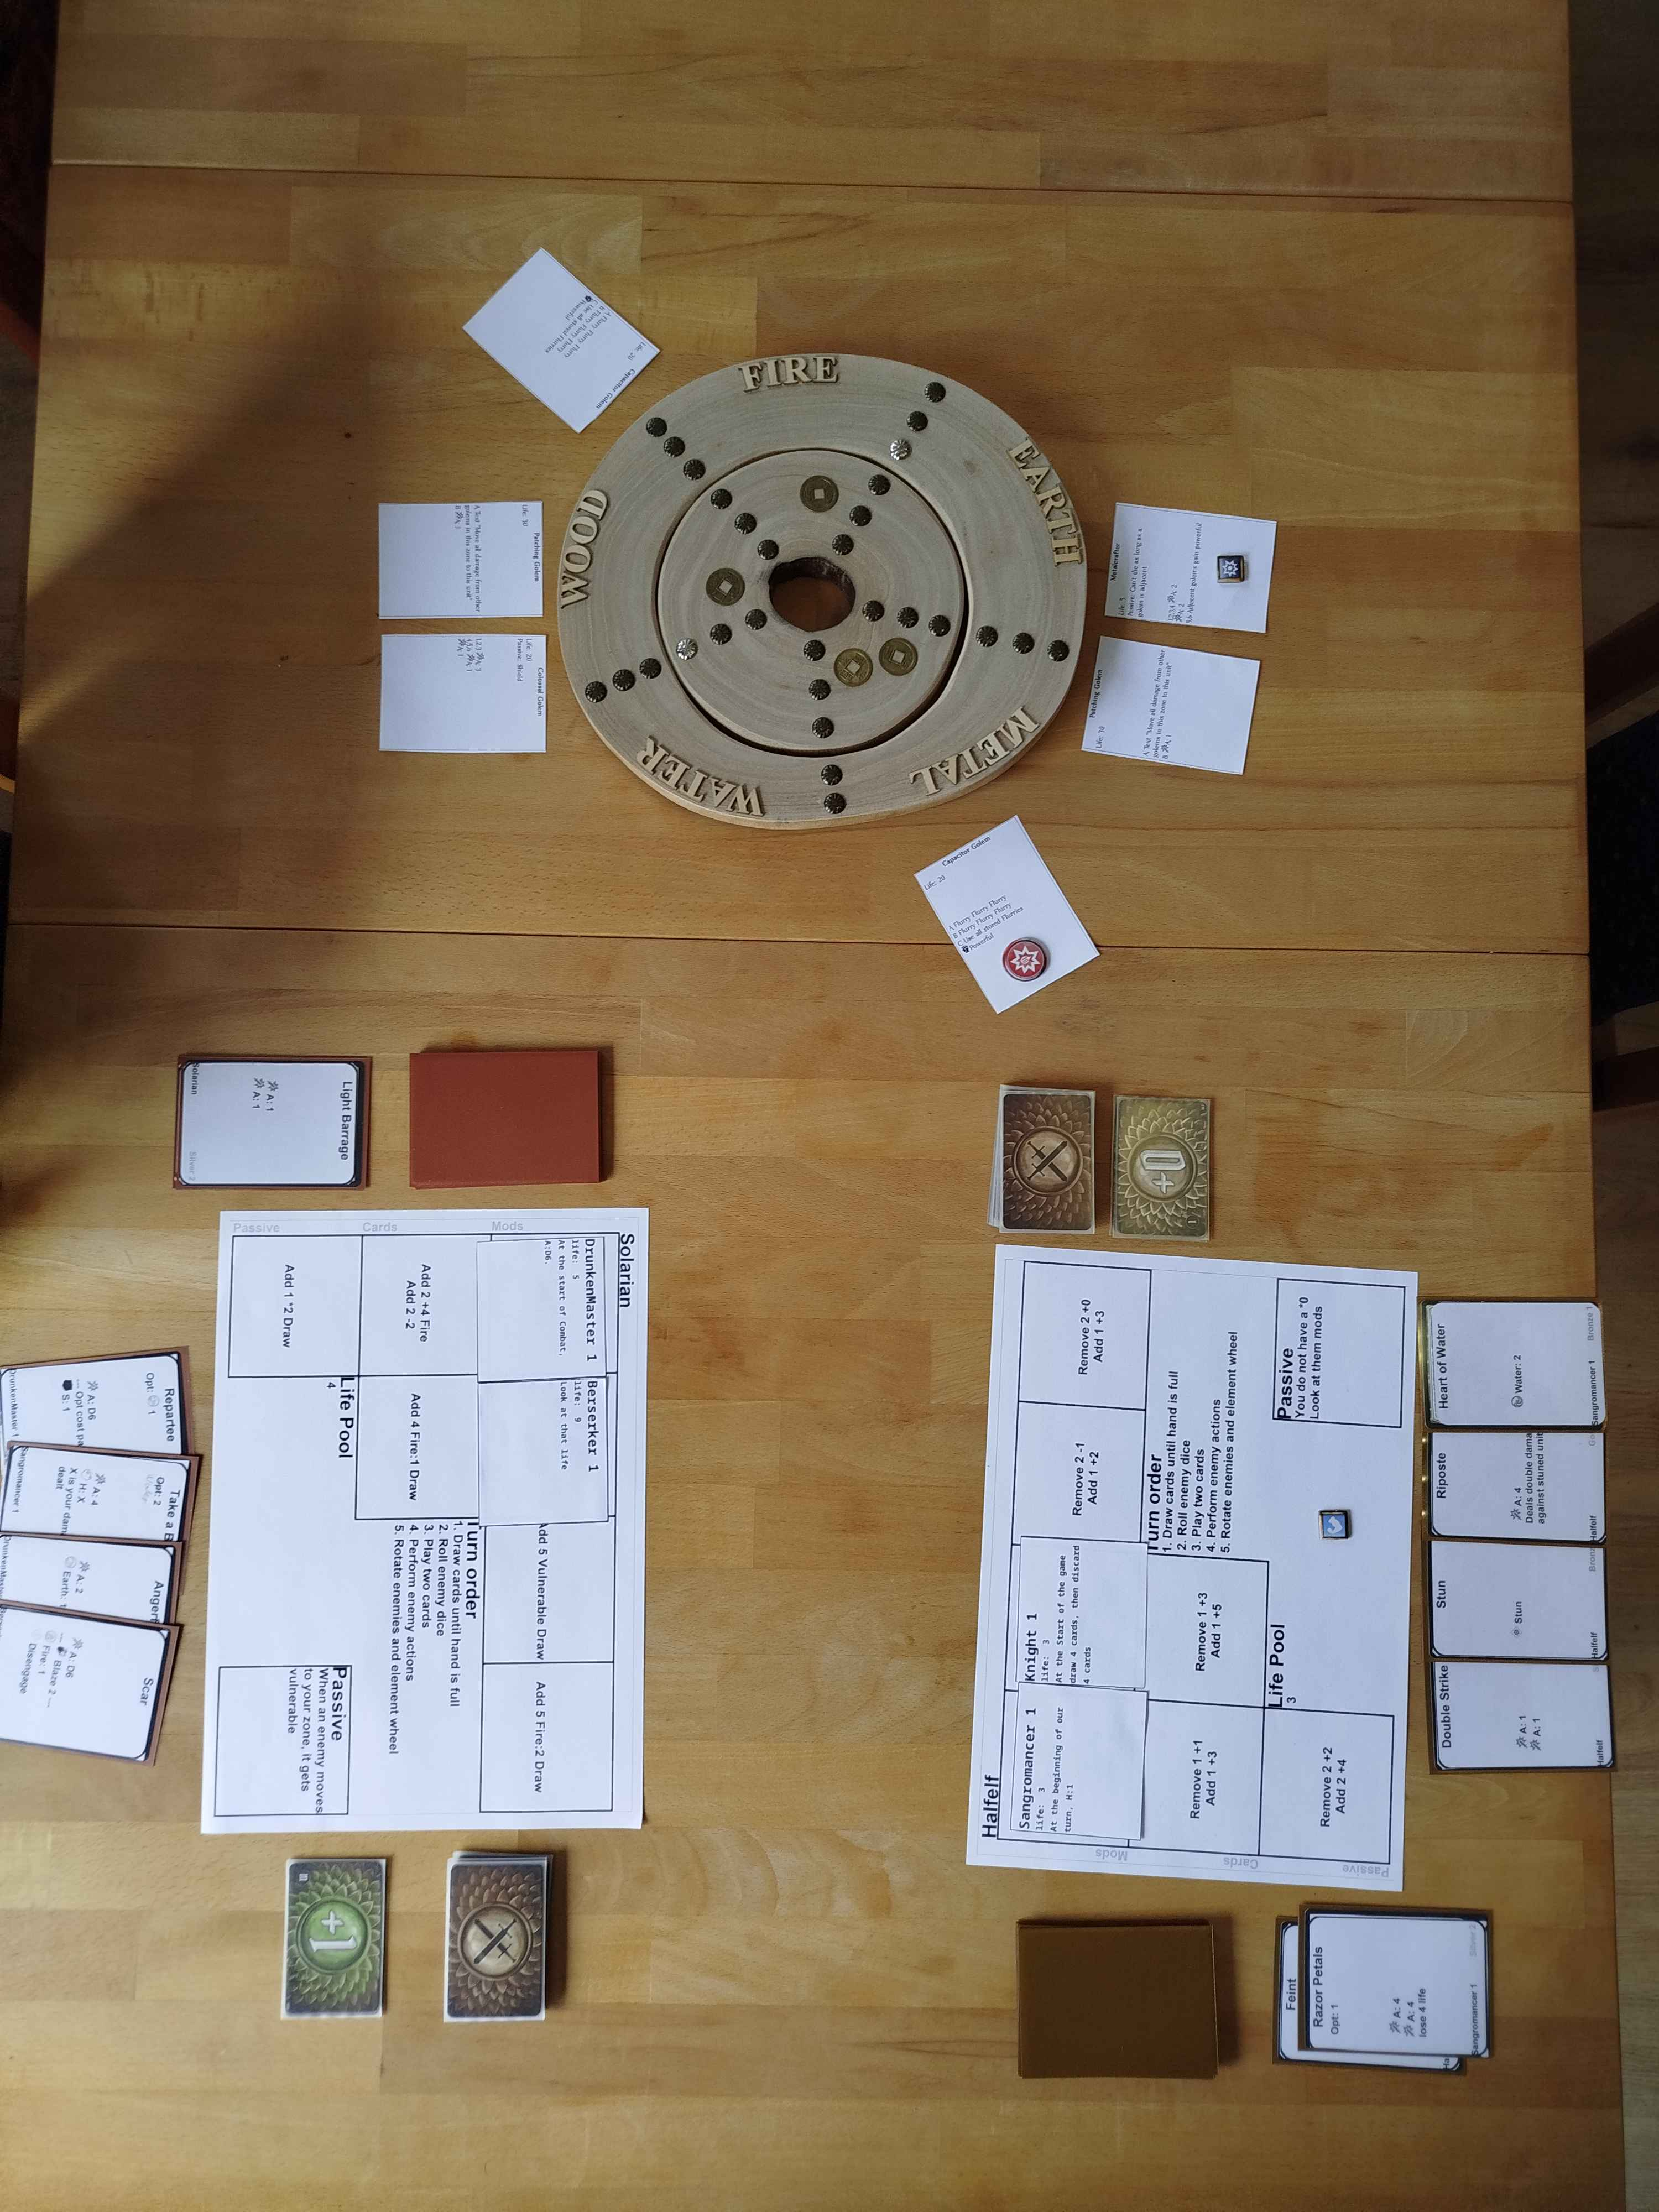
\includegraphics[width=0.8\textwidth]{../ExplanationPics/TwoBoards.jpg}





	
	
	
\subsection*{Setup for encounters 2 and 3}
After you beat an encounter, you level up \textit{(See "Leveling Up", Page \pageref{Section_Leveling})}.
Upgrade your decks with the cards from your new classes, and proceed to the next encounter by reading out the next part of the story and setting up the next enemies.
When you beat encounter 3, you win.
%After the first encounter, read out passage 2 from the storybook and set up the second encounter.
%When beating encounter 2, repeat with passage 3 and encounter 3, and when you beat encounter 3,  read the last passage from the story. When you reach this point, you win.

